\documentclass[11pt,a4paper]{article}
\usepackage{ls}
\usepackage[english]{babel}

\title{Solving problems with TRIZ and AIPS-2015}

\author{Hans-Gert Gr\"abe, Leipzig}

\date{10 April 2021}

\begin{document}
\maketitle

\subsection*{TRIZ and the World of Contradictions}

The TRIZ world is about contradictions in real existing technical systems (TS)
or TS to be designed. A TS has always to be considered in the unity of the
description form and the execution form. This unity is of a dialectical nature
in the sense of \cite{Graebe2020} -- in the description form unity in
diversity plays the central role, in the execution form the recovery of
diversity from unity is prevalent.  This abstract formulation is to be
understood as follows: From diversity abstract \emph{technical
  principles}\footnote{This term "principle" is not to be confused with the
  same word in the connotation as "TRIZ principle", which is an unfortunate
  translation of the Russian word "Prijom", and would be better translated as
  "procedure".} are derived and condensed in techno-scientific
\emph{procedures}.  In the executive form, on the other hand, \emph{several}
such procedures are used in interaction to solve a real-world technical
problem.  However, the latter is also accompanied by a description form, a
\emph{description form of second kind}, which is different and has to be
distinguished from description forms of first kind for domain-specific
technical principles, since they are about the \emph{interplay} of the
domain-specific technical principles in a real-world technical solution.

This distinction carries through up to professional profiles -- specific
technical procedures are developed by specialists, real-world technical
solutions by generalists, see in detail \cite[section 9]{Graebe2020}.
However, the world is not so dichotomously structured, but rather fractal.
Specialists in one perspective may as well be generalists in another
perspective, namely when we are faced with a domain-specific problem that
requires specialists from other domains to solve it.

\subsection*{TRIZ as a Methodology for Generalists}

In this sense, TRIZ is a methodology for generalists, who consult specialists
on individual questions. This team-player approach, which is very important
for the successful practical application of the methodology, is hardly
elaborated.  On the contrary, the TRIZ methodology is based on the central
concept of a "creative personality" and sees her in an important leading
position for the whole process of problem solving. Conflicting situations with
the management are dealt with more from a private-psychological and less from
a structural perspective.

TRIZ training is about methodically to support this generalist in his work. In
\emph{advanced TRIZ training} it is a matter of dealing with complex
requirement situations with a larger number of both of components as well as
contradictions, SF modelling, RCA, CECA and trends of evolution of TS as tools
to find one's way in a complex landscape of contradictions and to identify a
starting point for the solution of a given problem, where the skills of
problem analysis acquired in the \emph{TRIZ basic training} can be applied.

Common to both forms of training is the image of a pre-existing world of
strongly interdependent TS. Such a picture is based on description and
execution forms of \emph{direct} interaction between such systems and largely
ignores higher forms of abstraction such as framework models. This is due to
the fact that the TRIZ methodology itself is an interaction abstraction at
this level of analysis.  See \cite{Szyperski2002} for basic considerations on
such higher abstraction forms of "re-use".

Such a specific image of a generalist on the world of TS is assumed to be
constitutive for the TRIZ methodology.  In a first approach, TS are
delimitable \emph{Black boxes}, which in the description form are defined by
their \emph{specification} and in the execution form by their
\emph{specification compliant operation} provided that the operating
conditions of the TS are ensured by the infrastructure. These operating
conditions appear as import/export relations and are given in the description
form as \emph{purposes}, in the execution form as \emph{flows}, which manifest
themselves as \emph{throughputs} that are essential for the functioning of the
TS.

\begin{figure}[ht]\centering
  \includegraphics[width=.9\textwidth]{ARIZ-Workflow.png}\\
  \textbf{Figure 1:} The ARIZ-85C workflow in schematic representation
  according to I. Bukhman
\end{figure}

TRIZ basic training, the training objective of the TRIZ trainer \cite{TT},
addresses the general task to eliminate contradictory behaviour through a more
precise analysis of a \emph{single} critical system, without clear rules,
\emph{how} this critical system was identified in the first place.  This is
exactly how ARIZ-85C proceeds: At the end ("no answer or imperfect solution")
it says "Part 6: change or replace the problem. Back to Part 1". The
\emph{selection} of the critical system to be analysed in more detail is thus
largely heuristic and is, together with a first analysis of the internal
functioning of this system as a \emph{White Box}, the subject of the first
phase of the TRIZ trainer.  This essentially corresponds to Part 1 of
ARIZ-85C.  This has to be distinguished from the procedure in both the TRIZ
advanced training (such as PICC \cite{Cavallucci} by D. Cavallucci and his IDM
approach) as well as the procedure in more complex industrial application
situations, where further TRIZ instruments are used for this analysis.

\subsection*{The system and its Neighbouring Systems}

In a \emph{world of technical systems} there are actually no supersystems.
The prominent role of the supersystem-system relationship in the TRIZ
methodology has already been criticised in \cite[p. 16]{Graebe2020} and it has
been shown that this relationship is more or less identical with the
system-component relationship. I will return to this below.  In such a world
of systems, for a TS to be investigated such neighbouring systems are above
all essential which are in a close causal relationship to that TS.  It is to
be expected, especially after phases of \emph{trimming}, that \emph{several}
such neighbouring systems are causally important.  

In the TRIZ trainer \cite{TT} these relationships are reduced to the informal
determination of the \emph{purpose} and \emph{main useful function} (MUF) of a
previously delineated problematic technical system (TS) as determination of
its specification using a black-box approach.  Following an approach of
autonomy of the TS under investigation, its (external) operating conditions
are largely left out. The (methodical) approach can therefore not necessarily
be transferred to components, since according to the evolution law of "energy
conductivity"\footnote{"The continuous flow of energy through all parts of the
  system is a necessary condition for the basic viability of a technical
  system" \cite[p. 125]{Altshuller1983}. "The basic prerequisite for the
  viability of a system is the free flow of energy through all its parts."
  \cite[p. 172]{Koltze2017}. Somewhat differently \cite[p. 86]{TESE2018}: "The
  trend of Flow Enhancement is much more sophisticated, and it also takes
  substance and energy into account."  Recent versions also take information
  into account.} the flow of substance, energy and information through all of
its components is an essential property of the viability of a TS.

The tasks of the TRIZ trainer therefore basically refer to TS with a certain
autonomy status (boat in water traffic, truck in mining, racing driver in a
desert rally, etc.). On the other hand, since TRIZ works with a precise
localisation of contradictions, the component structure of the TS has to be
analysed in more detail, including the analysis of sub-components of different
hierarchical levels up to the localisation of the problematic component and
the operational zone.

\begin{figure}[ht]
  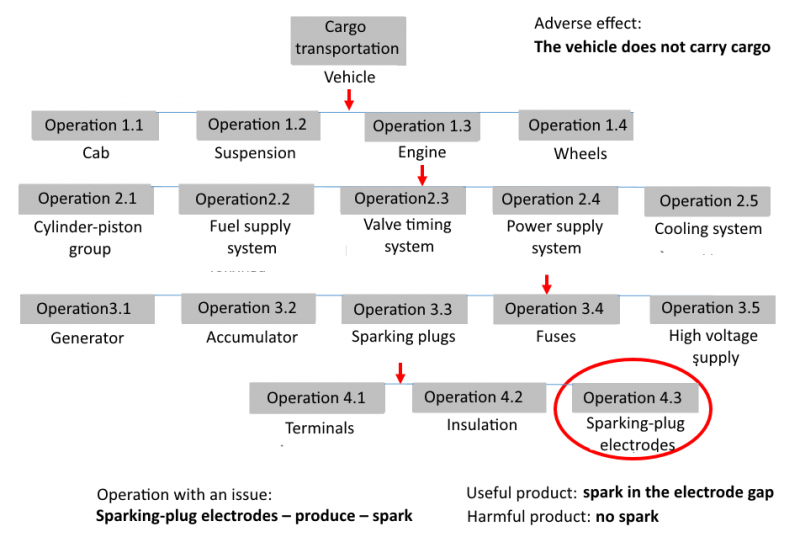
\includegraphics[width=.9\textwidth]{2918_xxl.png}\\
  \textbf{Figure 2:} Identification of the problematic component in the
  hierarchy of system components (from \cite{TT})
\end{figure}

Furthermore, the workflow organisation ("how the machine works" in \cite{TT})
of both the TS and the problematic component have to be analysed. The workflow
analysis of the system shows which resources are occupied by the system and
thus are primarily available or can be reallocated for problem solving. The
workflow analysis of the problematic component shows the structure of the
conflict and is the primary object of a "classical" TRIZ analysis. The
workflow analysis of the TS is, however, also helpful to develop an
appropriate notational framework for the analysis of the problematic
component, especially if, in the course of the workflow analysis of the TS, it
turns out that there are different states (operating state, maintenance state,
etc.), which appear as contextualising conditional patterns in the
determination of the operational time and thus "separation by change of
conditions" \cite[p. 111]{Koltze2017} can be applied.

\subsection*{TRIZ Trainer -- the Solution Process}

In the TRIZ trainer \cite{TT}, the algorithmic version AIPS-2015\footnote{AIPS
  is a Russian acronym and stands for "Algorithm of changing problematic
  situations".} of TRIZ is used, which is described in more detail in
\cite{TT}.  We assume the reader to be familiar with these concepts.

In a \textbf{first phase}, for the modelling of the conditions of the task
therefore must be identified
\begin{enumerate}[noitemsep]
\item the \emph{system} (using a "speaking name"), its \emph{purpose}, the
  \emph{PNF}, the required \emph{operating conditions}, and the
  \emph{problematic behavior} to be eliminated (section "Specification of
  circumstances"), 
\item the structural organisation of the system -- which components and which
  resources are used, where is the problem concentrated, recursive analysis of
  the structural organisation of sub-components as in figure 2 up to the
  \emph{operational zone} where the problem manifests itself -- (section
  "Machine"),
\item the workflow organisation of the system as a whole (preliminary work to
  identify resources that are available in the system to solve the problem)
  and of the problematic sub-component (section "Machine operation").
  
  The workflow organisation leads in many cases to a clear distinction of
  different \emph{states}, which should be taken into account for optimal
  solutions as different modes of operation of the system.  These states are
  to be clearly conceptualised and delineated in the section "machine
  operation".
\end{enumerate}

At the end of this analysis, the useful as well as the inadequate or harmful
actions are to be listed, if possible, as formalised statements "tool acts-on
object" (section "systemically relevant actions") and on this basis the
conflict (place, time, structure) has to be described in more detail as a
basis for planning a transformation of the system that solves the problem.

At the end of this first phase (in computer science also called
\emph{requirements analysis}) we build up an exact model of the TS.  Further
(section "proposing hypotheses"), on the basis of this detailed model, a
\emph{refined task} is to be formulated, solving it would solve the problem.
With the formulation of the task the \emph{direction} of the solution is
already clear at this point, even though the details still have to be worked
out in the further process.

For the specified hypothesis, in the \textbf{second phase of the solution
  process} one or more \emph{ideas for a solution} are to be found by
analysing the available resources. 

This second phase includes the following parts:
\begin{itemize}[noitemsep]
\item[(1)] Selection of a problem model that fits the conflict structure
  identified in the first phase.
\item [(2)] Identify, as comprehensively as possible, \emph{resources} which
  fit the problem model and the conflict structure.
\item [(3)] Selection of an appropriate TRIZ tool as a \emph{transformation
  method}.
\item [(4)] Configuration of the tool according to the specific
  conflict structure (\emph{solution model}).
\item [(5)] Instrumentation of the solution model with appropriate resources.
\end{itemize}
While (1) is associated with an essential methodological decision, steps
(2)-(5) are closely related. A coherent picture of the model often emerges
only after repeated back and forth, when later new insights have an influence
on earlier steps.  In most cases, it is discovered that the modelling was too
coarse or that essential aspects were overlooked. In such a case, the
modelling must be revised from that point on.

These refinements may also reveal that the first phase was insufficiently
elaborated or that the problem model does not fit.  In this case, the deeper
insights should be used to return to the first phase, the modelling there
should be clarified and thus the context will be adjusted, which is
constitutive for the second phase.  

At the end, in the \textbf{third phase}, one of the solution ideas is to be
elaborated in more detail as the \emph{final solution} and to be checked
whether the solution works.

\subsection*{External Components and Resources}

When modelling the TS under investigation as white box, it should be noted,
that it happens that it uses services from other systems via their interfaces.
Typically, these are components of the TS that are considered as a black box
within the system modelling, the ability of which is described by an interface
specification and whose practical performance is given by a specification
compliant \emph{throughput} through the system, which is constitutive for the
functioning of the TS. Hence the \emph{external} throughput keeping the TS
alive comes partially from the \emph{inside} of the TS.

When searching for resources with certain properties, for example as an
X-component, it is possible that external resources are subsequently to be
integrated into the system modelling (in the sense of the evolution law of
"increasing system completeness"). In a world of technical systems, these are
neighbouring components that were not previously part of the TS.  Hence, in
the course of system modelling, there is a natural process of transformation
of neighbouring components into system components to be taken into account.
Here, the structural similarity (descriptions of the of neighbouring
components are available as black boxes in the same way as of internal
components; and like them they can only be addressed via interface
specifications) substantiates a merging of the two "concepts" -- internal and
neighbouring component -- to a common notion of \emph{potentially available
  components}, at least for modelling purposes.

Since, on the other hand, the modelling of the internals of the system in the
section "system conflict" of the first phase in the TRIZ-Trainer is anyway
restricted to \emph{essentials} (essential components and essential relations)
according to a given methodological pattern (energy source, transmission,
tool, ..., control), there is no problem to include \emph{potentially all}
neighbouring systems as components in the modelling of the TS under
investigation and to include the relations between them as relations between
components.  The originally largely arbitrary delimitation of the "autonomous
TS" reads in this way as (initial) weighting of components and relationships
according to a principle of "essentiality" given by the modelling purpose.

This is, of course, a formal step that is largely transparent to the TRIZ
novice, which starts with the selection of those components and relationships
in APIS-2015 that are \emph{essential} according to the inner logic of the
system.  However, the methodological advantage is, that the system to be
modelled \emph{in such a modelling context} has no longer an outer side and
thus is more homogeneous.

In APIS-2015, a shell model is proposed for the search for resources to
instrumentalise the solution model that includes step by step
\begin{enumerate}[noitemsep]
\item the operative zone with tool and processed object,
\item system components in the environment of the operative zone,
\item system components at all (i.e. those already identified as part of the
  system in the previous modelling),
\item readily available resources from the environment (the "upper system"),
\item machine components (which is redundant in a certain sense) and
\item environmental components.
\end{enumerate}
The distinction between resources and components remains vague in that
respect, resources being the more general term and also include "natural"
resources, although every resource being useful in the system also has a (even
rudimentary) \emph{description} of its "usefulness" properties in the form of
a black-box model. In this respect, the terms differ only gradually.

For the search for resources, a good functional analysis \cite[sec.
  4.4]{Koltze2017} is important in order to describe the required
characteristics of the resource as precisely as possible.  In advanced
applications, the opposite is also helpful, namely the exact knowledge of the
properties of resources in an \emph{effect database} as explained in
\cite[sec.  8.2]{Koltze2017} in more detail as well as the potential of a
\emph{function-oriented search} as described in \cite[sec.  4.14]{Koltze2017}
which specifically searches for more precisely specified functionalities of
the same type in other technology areas.

\bibliographystyle{plain}
\begin{thebibliography}{xxx}
\bibitem{Altshuller1983} Genrich S. Altshuller (1983). Wings for Icarus.
\bibitem{Cavallucci} Denis Cavallucci. PICC Solutions. Augmented Human
  Intelligence.  \url{https://www.picc-solution.com/}
\bibitem{Graebe2020} Hans-Gert Gräbe (2020). People and their technical
  Systems (in German). LIFIS Online, Mai 2020.
  \url{doi:10.14625/graebe_20200519}
\bibitem{Koltze2017} Karl Koltze, Valeri Souchkov (2017). Systematic
  Innovation methods (in German). Hanser, Munich.
\bibitem{TESE2018} Alex Lyubomirskiy, Simon Litvin, Sergei Ikovenko et al.
  (2018). Trends of Engineering System Evolution (TESE).  TRIZ Consulting
  Group.  ISBN 9783000598463.
\bibitem{Szyperski2002} Clemens Szyperski (2002). Component Software. Addison
  Wesley, Boston. 
\bibitem{TT} TRIZ-Trainer. \url{https://triz-trainer.com}.
\end{thebibliography}

\end{document}
